\documentclass[a4paper,12pt]{article}

\usepackage[utf8]{inputenc}
\usepackage[czech]{babel}
\usepackage[IL2]{fontenc}
\usepackage[left=3cm,text={15cm, 23cm},top=3.5cm]{geometry}
\usepackage{subcaption}
\usepackage{listings}

\usepackage{color}
%\usepackage[unicode,plainpages=false,pdftex]{hyperref}
\usepackage[ruled,czech,linesnumbered,noline]{algorithm2e}
%\usepackage[dvipdf]{graphicx}
\usepackage{graphicx}

\usepackage{tikz}
\usetikzlibrary{patterns}

\definecolor{grey}{rgb}{0.745098,0.745098,0.745098}

\lstset{ %
  basicstyle=\scriptsize
}

\usepackage{amssymb}
\usepackage{amsmath}
\usepackage{amsthm}
%	\usepackage{graphicx}

\usepackage{tikz}

\title{Projekt do předmětu FAV -- Nástroj CPAchecker}
\author{Vojtěch Havlena, xhavle03}

\begin{document}
\maketitle

\section{Charakteristika nástroje}
\textsc{CPAchecker} je volně dostupný framework a konfigurovatelný nástroj pro softwarovou verifikaci programů napsaných v jazyce C.
V tomto projektu jsem využil verzi 1.4 pro operační systém Linux.
Samotný nástroj je napsán v jazyce Java\footnote{pro běh je nutný Java Runtime Environment verze 7+} a je vyvýjen na univerzitě v německém Passau. Nástroj \textsc{CPAchecker} je založen na 
konceptu konfigurovatelné analýze programů (configurable program analysis -- CPA).
CPA je koncept, který umožňuje pomocí stejného formálního základu vyjádřit různé verifikační přístupy. Tedy pomocí jediného
formalismu je možné vyjádřit různé přístupy založené na analýze programů a na model checkingu \cite{cpa}. 

\subsection{Základní vlastnosti}
\textsc{CPAchecker} je nástroj zahrnující model checking, založený na predikátové abstrakci (implementováno jako CPA, viz. níže). V mnoha 
ohledech je \textsc{CPAchecker} podobný nástroji \textsc{Blast}\,--\,pro predikátovou analýzu se stejně jako v 
nástroji \textsc{Blast} využívá lazy abstrakce a interpolace~\cite{cpa}. Výhodou nástroje \textsc{CPAchecker} je jeho snadná konfigurovatelnost.
Nástroj může například provádět predikátovou analýzu použitím single-block encoding (SBE), large-block encoding (LBE), popřípadě
adjustable-block encoding (ABE). O přístupu single-block encoding hovoříme v případě, kdy hrana v abstract reachibility graph (ARG)
reprezentuje jeden blok v programu. V případě, že hrany v ARG reprezentují větší část programu, hovoříme o LBE~\cite{lbe}. ABE potom
umožňuje vyjádřit oba předchozí přístupy. 

Další výhodou, především
oproti nástrojům, které implementují smyčku abstract-check-refine odděleně je, že on-the-fly přístup lazy abstrakce umožňuje 
použití efektivnějších a flexibilnějších algoritmů. Do nástroje \textsc{CPAchecker} je také integrován bounded
model checker pro kontrolu proveditelnosti chybových cest. Je rovněž využíván přístup CEGAR.

\subsection{Architektura}
Celý nástroj \textsc{CPAchecker} se skládá z několika částí. V první části se vstupní program ve zdrojovém kódu
převede do syntaktického stromu. Na základě tohoto stromu se potom vytvoří control-flow automaty, které reprezentují program~\cite{cpa}. 
Z těchto automatů se potom postupně buduje abstract reachibility graph (ARG).

Jádrem 
celého nástroje je CPA algoritmus~\cite{alg}. CPA algoritmus provádí analýzu dosažitelnosti s tím, že pracuje nad objekty abstraktního
datového typu CPA. CPA tedy tvoří rozhraní pro operace, které jsou využívány v CPA algoritmu, který nad těmito operacemi
pracuje bez znalosti jejich konkrétní implementace. Konkrétní použitý CPA může být také kombinací více různých CPA (v tom případě
se hovoří o složené CPA)~\cite{cpa}. \textsc{CPAchecker} obsahuje konkrétní implementaci CPA např. pro predikátovou abstrakci. Stručné schéma
celého nástroje je na obr.~\ref{fig:sch}.

\begin{figure}[h!]
\begin{center}
\begin{tikzpicture}[every text node part/.style={align=center}]
  \draw (0,0) rectangle (1.5,2);
  \draw (4,1) ellipse (1.2 and 0.75);
  \draw (7,1) ellipse (1.2 and 0.75);
  \draw (10,1) ellipse (1.2 and 0.75);
  \draw (12.5,0) rectangle (14.5,2);
  
  \draw[->,thick] (1.6,1) -- (2.7,1);
  \draw[->,thick] (5.3,1) -- (5.7,1);
  \draw[->,thick] (8.3,1) -- (8.7,1);
  \draw[->,thick] (11.3,1) -- (12.4,1);
  
  \draw node at (4,1) {{\small\sf Parser}};
  \draw node at (7,1) {\small\sf CFA\\ \sf Builder};
  \draw node at (10,1) {\small\sf CPA\\ \sf Algoritmus};
  \draw node at (0.75,1) {\small\sf Zdroj.\\ \sf kód};
  \draw node at (13.5,1) {\small\sf Výsledek\\ \sf verifikace};
  
  \draw (6.9,2.4) rectangle (8.6, 3.6);
  \draw (8.9,2.4) rectangle (10.6, 3.6);
  \draw (10.9,2.4) rectangle (12.6, 3.6);
  
  \draw[->,thick] (9.5,1.75) -- (7.75,2.3);
  \draw[->,thick] (10,1.85) -- (9.75,2.3);
  \draw[->,thick] (10.5,1.75) -- (11.75,2.3);
  
  \draw node at (7.75, 3) {\small\sf Octagon\\ \sf CPA};
  \draw node at (9.75, 3) {\small\sf Explicit\\ \sf CPA};
  \draw node at (11.75, 3) {\small\sf Predicate\\ \sf CPA};
\end{tikzpicture}
\end{center}
\caption{Schéma nástroje \textsc{CPAchecker}. Převzato a upraveno z~\cite{cpa}}
\label{fig:sch}
\end{figure}

V případě rozšíření nástroje \textsc{CPAchecker} o další CPA pro novou abstraktní doménu, je nutné provést následující
kroky. Nejprve je nutné pro nový CPA vytvořit záznam v globálním konfiguračním souboru. Dále je nutné, aby nový CPA 
implementoval požadované CPA rozhraní a všechny operace v něm obsažené. Například pokud chceme implementovat CPA
pro shape analýzu, vytvoříme nový CPA obsahující konkrétní implementaci operací. Je možné také vytvořit několik
různých implementací stejné operace pro daný CPA~\cite{cpa}.

\subsection{Použití}
Nástroj \textsc{CPAchecker} provádí analýzu programů zapsaných v jazyce C. Podle vývojářů je nástroj schopný parsovat
a analyzovat velkou podmnožinu jazyka (GNU) C. Před samotnou verifikací je nutné provést předzpracování vstupního zdrojového kódu 
preprocesorem jazyka C\,--\,zdrojový kód nesmí obsahovat direktivy \texttt{\#define} a \texttt{\#include} (případně lze využít 
přepínač \texttt{-preprocess} a \textsc{CPAchecker} sám toto předzpracování provede). \textsc{CPAchecker} také experimentálně
poskytuje možnost spojit více C souborů a provést nad nimi verifikaci.

Specifikace pro verifikaci se zadává pomocí jednoduchého automatu (jazyk pro popis těchto automatů je podobný jazyku \textsc{Blast} 
Query Language~\cite{bql}). S nástrojem jsou dodávány i již předdefinované specifikace.
Specifikace je vyjádřena pomocí vlastností dosažitelnosti (ve výchozí specifikaci to je kontrola příkazu \texttt{assert}, dosažení labelu \texttt{ERROR} a volání funkcí
\texttt{abort()} a \texttt{exit()}). 

Pro běh nástroje \textsc{CPAchecker} se nejčastěji používá kombinace specifikace konfiguračního souboru pro verifikaci (přepínač 
\texttt{-config}, definuje parametry verifikace, ověřovanou specifikaci apod.) a samotného souboru se zdrojovým textem, který se 
má verifikovat. Výběr vhodné konfigurace záleží na konkrétní podobě programu, který se má verifikovat.
Mezi předdefinované přepínače zastupující konfigurační soubory mj. patří:
\begin{itemize}
 \item \texttt{-predicateAnalysis} -- predikátová analýza s přístupem CEGAR, doporučeno pro obecné použití
 \item \texttt{-valueAnalysis} -- analýza hodnot (value analysis) celočíselných proměnných
 \item \texttt{-bmc-induction} -- bounded model checking, použití indukce pro dokázání bezpečnosti. Tato konfigurace
   je zatím označena jako experimentální.
 \item A další (\texttt{-sv-comp15}, \texttt{-octagonAnalysis},  \dots)
\end{itemize}

Nevýhodou nástroje \textsc{CPAchecker} je nepodporování verifikace programů, které obsahují rekurzi (existuje
ale nástroj založený na \textsc{CPAchecker}u, nazvaný \textsc{CPArec}, který umožňuje verifikaci rekurzivních C programů). 
Dále \textsc{CPAchecker} nepodporuje verifikaci programů obsahující souběžnost. Další nevýhodou je absence tutoriálu,
popřípadě nějaké podrobnější uživatelské dokumentace k používání nástroje.

I přesto se tento nástroj v praxi používá (používá jej např. výzkumná skupina zabývající se verifikací Linuxových
ovladačů). Pomocí tohoto nástroje bylo také odhaleno několik chyb v Linuxovém jádře. Navíc na 
soutěži Competition on Software verification se nástroj \textsc{CPAchecker} v určitých kategoriích pravidelně 
umísťuje na čelních pozicích\footnote{viz. \texttt{http://sv-comp.sosy-lab.org/2015/results/}}.

\section{Experimenty na stávajících příp. studiích}
Spolu s nástrojem jsou dodávány různé zdrojové soubory v jazyce C, které byly použity např. pro srovnávací experimenty
s jinými nástroji. Na těchto souborech je možné vyzkoušet běh nástroje \textsc{CPAchecker}. Po ukončení běhu je vygenerován
soubor se shrnujícími informacemi a statistikami o proběhlé verifikaci. Všechny experimenty jsem prováděl na systému
GNU/Linux (Debian 8) 64 bit, 4-jádrový procesor AMD, 6\,GB RAM.

Asi nejjednodušším
z těchto dodávaných souborů je \texttt{example.c}, který obsahuje funkci \texttt{main}, dvě celočíselné proměnné, cyklus while a několik podmínek. Chybový 
stav je označen návěštím \texttt{ERROR}. Zdrojový soubor neobsahuje direktivy preprocesoru, není tedy nutné používat parametr \texttt{-preprocess}. 
Vzhledem k použitému chybovému návěští, jsem zvolil výchozí specifikaci, která obsahuje dosažení labelu \texttt{ERROR}. 
Samotnou verifikaci jsem potom provedl s následujícími konfiguracemi:
\begin{itemize}
 \item \texttt{-predicateAnalysis}. Pro tuto konfiguraci verifikace skončila, vzhledem k zadané specifikaci, s výsledkem \textsc{Safe}.
 Běh trval 2.75\,s. Množství využité paměti hromady je 47\,MB. Soubor se statistikami obsahuje i další podrobnější informace
 o verifikaci a využitých zdrojích během verifikace -- počet abstrakcí: 5, zdroje využité pro BDD (počet uzlů BDD: 205, \dots), statistiky algoritmu 
 CEGAR (počet zpřesnění: 1, \dots), apod.
 
 \item \texttt{-valueAnalysis}. Pro tuto konfiguraci opět verifikace skončila s výsledkem \textsc{Safe}. Běh trval 2.46\,s. Množství využité 
 paměti hromady je 48\,MB.
 
 \item \texttt{-bmc-induction}. Výsledek verifikace byl opět \textsc{Safe}. Při této konfiguraci běh trval 3.46\,s.
 Množství využité paměti hromady je 43\,MB
 
 \item \texttt{-sv-comp15}. Pro tuto konfiguraci bylo nutné provést úpravu konfiguračního souboru tak, aby bylo povoleno 
 vytváření statistiky. Výsledek verifikace byl opět \textsc{Safe}. Běh trval 2.20\,s a množství využité paměti hromady
 je 50\,MB.
\end{itemize}
Pomocí dodávaného skriptu je také možné vygenerovat control-flow automaty a abstract-reachibility graf, které byly vytvořeny 
ze zdrojového textu během procesu verifikace. Příklad CFA pro zdrojový soubor \texttt{example.c} je na obr.~\ref{fig:cfa}. Skript také 
umožňuje celý výsledek verifikace přehledně zobrazit v HTML souboru. V případě, že vstupní 
program obsahuje chybu, je v CFA a ARG vyznačena cesta, která vedla k chybě.

\begin{figure}[h!]
 \centering
 \includegraphics[scale=0.3]{Images/cfa__main.png}
 \caption{CFA použitý při verifikaci souboru \texttt{example.c}.}
 \label{fig:cfa}
\end{figure}

Kromě verifikace tohoto jednoduchého programu jsem provedl verifikaci na dalších dodávaných programech. Experimentoval
jsem na jedné z dodávaných sadách benchmarků. Sada, kterou jsem použil, tvoří zjednodušené ovladače v systému Windows.
Kromě této sady je k dispozici např. sada, obsahující zjednodušené verze stavových automatů, které zabezpečují komunikaci v rámci SSH. Pro všechny provedené
experimenty byla použita výchozí specifikace. Pro verifikaci jsem nejprve zvolil konfigurace \texttt{-predicateAnalysis} (predikátová analýza) a
\texttt{-valueAnalysis} (analýza hodnot). Dodávané zdrojové soubory již neobsahují direktivy preprocesoru, není je tedy nutné upravovat. Verifikované
programy jsou již komplexnější programy, obsahují podstatně více celočíselných proměnných, cyklů, podmínek a funkcí než základní soubor \texttt{example.c}. Samotné výsledky 
těchto experimentů lze nalézt v tabulce~\ref{tab:res1}. V případě, že byla nalezena chyba,
ve vygenerovaném CFA byla vyznačena cesta k této chybě. Výsledné CFA s chybou zde ale kvůli rozměru neuvádím.

\noindent
\begin{table}[h!]
\renewcommand{\arraystretch}{1.2}
\begin{center}
  \begin{tabular}{| l | p{1.7cm} | c  c  c | c  c  c |}
    \hline
    \multicolumn{1}{|c|}{\bf Program} & {\small\bf Oček.} & \multicolumn{3}{c|}{\small\bf -predicateAnalysis} & \multicolumn{3}{c|}{\small\bf -valueAnalysis}  \\
     & {\small\bf výsledek}  & Výsl. & Čas\,[s] & Paměť & Výsl. & Čas\,[s] &  Paměť\\
    \hline\hline
    {\small \texttt{cdaudio\_simpl1}} & \textsc{Safe} & \textsc{Safe} & 19.46 & 117 & \textsc{Safe} & 19.85 & 407  \\ \hline
    {\small \texttt{cdaudio\_simpl1\_BUG}} & \textsc{Bug} & \textsc{Bug} & 16.01 & 141 & \textsc{Bug} & 10.19 & 199  \\ \hline
    {\small \texttt{diskperf\_simpl1}} & \textsc{Safe} & \textsc{Safe} & 12.78 & 112 & \textsc{Safe} & 13.67 & 380  \\ \hline
    {\small \texttt{floppy\_simpl3}} & \textsc{Safe} & \textsc{Safe} & 10.55 & 110 & \textsc{Safe} & 11.09 & 300 \\ \hline
    {\small \texttt{floppy\_simpl3\_BUG}} & \textsc{Bug} & \textsc{Bug} & 12.74 & 110 & \textsc{Bug} & 12.24 & 327  \\ \hline
    {\small \texttt{floppy\_simpl4}} & \textsc{Safe} & \textsc{Safe} & 11.26 & 108 & \textsc{Safe} & 12.69 & 374 \\ \hline
    {\small \texttt{floppy\_simpl4\_BUG}} & \textsc{Bug} & \textsc{Bug} & 13.46 & 113 & \textsc{Bug} & 13.17 & 375  \\ \hline
    {\small \texttt{kbfiltr\_simpl1}} & \textsc{Safe} & \textsc{Safe} & 4.80 & 60 & \textsc{Safe} & 6.62 & 103  \\ \hline
    {\small \texttt{kbfiltr\_simpl2}} & \textsc{Safe} & \textsc{Safe} & 5.95 & 59 & \textsc{Safe} & 7.36 & 105 \\ \hline
    {\small \texttt{kbfiltr\_simpl2\_BUG}} & \textsc{Bug} & \textsc{Bug} & 8.02 & 75 & \textsc{Bug} & 8.79 & 110  \\
    \hline
  \end{tabular}
\end{center}
\caption{Výsledek verifikace dodávaných souborů (zjednodušené ovladače systému Windows) pro konfigurace \texttt{-predicateAnalysis} a \texttt{-valueAnalysis}.
Pro každou konfiguraci a soubor je uveden výsledek verifikace, doba v sekundách a využitá paměť hromady v MB.}
\label{tab:res1}
\end{table}

Kromě výše zmíněných konfigurací jsem provedl experimenty také s konfigurací \texttt{-bmc-inductive}. Výsledky
experimentu jsou uvedeny v tabulce~\ref{tab:res2}. V případě, že byla v programu chyba, \textsc{CPAchecker}
ji sice odhalil (vypsal, že v programu existuje chyba), ale již se nepodařilo vytvořit chybovou cestu. Tudíž verifikace skončila s výsledkem \textsc{Safe}.
Toto chování může být způsobeno tím, že konfigurace \texttt{-bmc-indu\\ctive} je zatím označena jako experimentální a tudíž ne vše
může být funkční.


\begin{table}[h!]
\renewcommand{\arraystretch}{1.2}
\begin{center}
  \begin{tabular}{| l | p{2cm} | c  c  c |}
    \hline
   \multicolumn{1}{|c|}{\bf Program} & {\small\bf Oček.} & \multicolumn{3}{c|}{\small\bf -bmc-inductive}  \\
     & {\small\bf výsledek}  & Výsl. & Čas\,[s] & Paměť \\
    \hline\hline
    {\small \texttt{cdaudio\_simpl1}} & \textsc{Safe} & \textsc{Safe} & 10.41 & 113 \\\hline
    {\small \texttt{cdaudio\_simpl1\_BUG}} & \textsc{Bug} & \textsc{Safe} & 8.89 & 113 \\ \hline
    {\small \texttt{diskperf\_simpl1}} & \textsc{Safe} & \textsc{Safe} & 7.04 & 109 \\ \hline
    {\small \texttt{floppy\_simpl3}} & \textsc{Safe}  & \textsc{Safe} & 6.60 & 108 \\ \hline
    {\small \texttt{floppy\_simpl3\_BUG}} & \textsc{Bug} & \textsc{Safe} & 6.60 & 108 \\ \hline
    {\small \texttt{floppy\_simpl4}} & \textsc{Safe} & \textsc{Safe} & 7.07 & 106 \\ \hline
    {\small \texttt{floppy\_simpl4\_BUG}} & \textsc{Bug} & \textsc{Safe} & 7.44 & 109 \\ \hline
    {\small \texttt{kbfiltr\_simpl1}} & \textsc{Safe} & \textsc{Safe} & 4.66 & 61 \\ \hline
    {\small \texttt{kbfiltr\_simpl2}} & \textsc{Safe} & \textsc{Safe} & 5.51 & 58 \\ \hline
    {\small \texttt{kbfiltr\_simpl2\_BUG}} & \textsc{Bug} & \textsc{Safe} & 6.11 & 58 \\
    \hline
  \end{tabular}
\end{center}
\caption{Verifikace dodávaných souborů s konfigurací \texttt{-bmc-inductive}.}
\label{tab:res2}
\end{table}

\section{Experimenty na vlastních příp. studiích}
Vlastní experimenty jsem provedl na programu pracující s polem celočíselných hodnot. Program provádí řazení pole pomocí 
jednoduchého algoritmu selection sort. Zdrojový kód v jazyce C je uveden níže.

\lstinputlisting[language=C]{sortArray.c}

Nejprve se pole hodnot naplní celočíselnými hodnotami. Následně se pole seřadí pomocí algoritmu
selection sort. V posledním cyklu \texttt{for} je kontrola, zda je pole opravdu seřazeno v sestupném
pořadí hodnot. V rámci experimentu jsem postupně zvyšoval konstantu \texttt{n} a prováděl verifikaci.
Vzhledem k použitému labelu \texttt{ERROR} jsem použil výchozí specifikaci. Co se týče konfigurací, 
nejprve jsem použil \texttt{-valueAnalysis} a \texttt{-predicateAnalysis-bitprecise}. Nicméně při použití této konfigurace byl výsledek verifikace
\textsc{Unknown}, proto jsem další experimenty prováděl s konfigurací \texttt{-predicateAnalysis}.
CFA použitý při verifikaci je na obr.~\ref{fig:cfasort}.
Výsledky verifikace při této konfiguraci jsou potom uvedeny v tabulce~\ref{tab:selSort}.

\begin{figure}[h!]
 \centering
 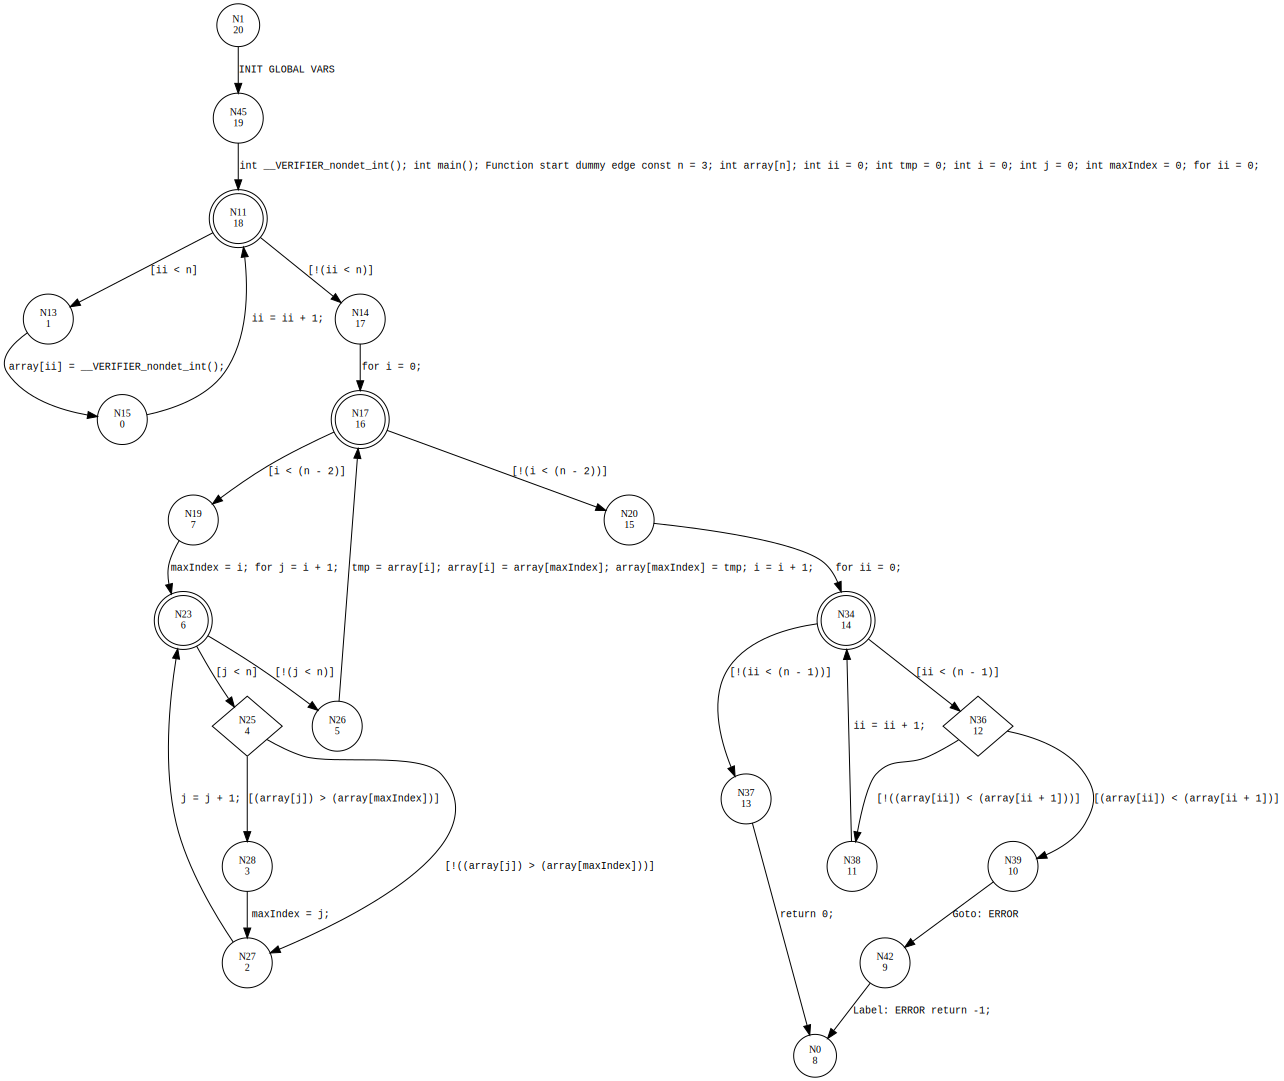
\includegraphics[scale=0.27]{Images/sortArray.png}
 \caption{CFA použitý při verifikaci řazení pole pomocí selection sortu.}
 \label{fig:cfasort}
\end{figure}

\begin{table}[h!]
\renewcommand{\arraystretch}{1.2}
\begin{center}
  \begin{tabular}{| c | c  c  c |}
    \hline
   \multicolumn{1}{|c|}{\bf Konstanta \texttt{n}} & \multicolumn{3}{c|}{\small\bf -predicateAnalysis}  \\
     &  Výsledek & Čas\,[s] & Paměť\,[MB] \\
    \hline\hline
    {\texttt{1}} & \textsc{Safe} & 4.32 & 48 \\\hline
    {\texttt{2}} & \textsc{Safe} & 6.94 & 59 \\ \hline
    {\texttt{3}} & \textsc{Safe} & 15.69 & 108 \\ \hline
    {\texttt{4}} & \textsc{Safe} & 47.08 & 205 \\ \hline
    {\texttt{5}} & \textsc{Unknown} & \textsc{To} & -- \\
    \hline
  \end{tabular}
\end{center}
\caption{Výsledky verifikace pragramu provádějící řazení staticky alokovaného pole, pro různé hodnoty konstanty \texttt{n}. Při verifikaci s konstantou \texttt{n = 5} vypršel časový limit, který 
byl nastaven na 900s.}
\label{tab:selSort}
\end{table}

Nyní se budu zabývat situací, kdy do programu zavedu chybu. Například, že 12. řádek původního programu nahradím za následující kód
\begin{lstlisting}[language=C]
   for(i = 0; i < n-2; i++),
\end{lstlisting}
tedy poslední prvek pole není zařazen na správné místo a pole nemusí být seřazené. V tomto případě při verifikaci s 
konfigurací \texttt{-predicateAnalysis} je obdržen výsledek \textsc{Bug} v čase 9.71\,s. 

V rámci dalšího experimentu jsem provedl modifikaci původního programu tak, aby pracoval s dynamicky alokovaným polem místo se statickým polem.
Tedy 5. řádek původního programu jsem zaměnil za následující kód
\begin{lstlisting}[language=C]
   int *array = (int *)malloc(n * sizeof(int));
   if(array == NULL)
      return 0;
\end{lstlisting}
Vzhledem k použití knihovní funkce \texttt{malloc} je nutné přidat i hlavičkový soubor \texttt{\#include<stdlib.h>}.
Při verifikaci je potom ale nutné použít přepínač \texttt{-preprocess}, protože v kódu je použita direktiva \texttt{\#include}.
Pro verifikaci jsem opět použil standardní specifikaci spolu s konfigurací \texttt{-predicateAnalysis} (stejně jako v předchozím
experimentu). Na řádku zdrojového kódu programu, který provádí alokaci pole je použito explicitní přetypování \texttt{(int *)}. V
případě, že bych toto přetypování nepoužil, \textsc{CPAchecker} při verifikaci objeví chybu. Experiment opět
spočíval ve verifikaci modifikovaného programu pro různé konstanty \texttt{n}. Výsledky experimentu jsou shrnuty
v tabulce~\ref{tab:mem}.

\begin{table}[h!]
\renewcommand{\arraystretch}{1.2}
\begin{center}
  \begin{tabular}{| c | c  c  c |}
    \hline
   \multicolumn{1}{|c|}{\bf Konstanta \texttt{n}} & \multicolumn{3}{c|}{\small\bf -predicateAnalysis}  \\
     &  Výsledek & Čas\,[s] & Paměť\,[MB] \\
    \hline\hline
    {\texttt{1}} & \textsc{Safe} & 4,78 & 57 \\\hline
    {\texttt{2}} & \textsc{Safe} & 7.62 & 71 \\ \hline
    {\texttt{3}} & \textsc{Safe} & 7.76 & 75 \\ \hline
    {\texttt{4}} & \textsc{Safe} & 10.52 & 111 \\ \hline
    {\texttt{5}} & \textsc{Safe} & 29.16 & 204 \\ \hline
    {\texttt{6}} & \textsc{Safe} & 45.27 & 381 \\
    \hline
  \end{tabular}
\end{center}
\caption{Výsledky verifikace pragramu provádějící řazení dynamicky alokovaného pole, pro různé hodnoty konstanty \texttt{n}}
\label{tab:mem}
\end{table}

Z tabulky plyne, že při použití dynamicky alokovaného pole v programu je doba běhu nástroje \textsc{CPAchecker} pro danou konstantu \texttt{n} nižší než při použití
staticky alokovaného pole. Paměťové nároky jsou v obou případech srovnatelné.

\section{Závěr}
Tato esej shrnuje poznatky získané při používání a studiu nástroje \textsc{CPAchecker}. V první části práce je
popsán princip, na kterém je nástroj postaven. Druhá část je věnována experimentům na existujících
případových studiích. Na existujících programech jsem experimentoval s verifikací pro různé konfigurace. Poslední část 
je potom věnována vlastním případovým studiím, kde je věnována pozornost verifikaci programu provádějící řazení celých čísel.

\bibliographystyle{czplain}
\bibliography{literatura}{}

\end{document}